%Package Date: 2018-01-01 % !TeX program = XeLaTeX

\documentclass[12pt]{report} \usepackage {preamble}

\title {\textbf{\huge Vulkan Unveiled: A Beginner's Guide to Professional
		Graphics Programming}} \author {Nick Schefner}
\bibliography{citations.bib}

\begin {document} \maketitle

\tableofcontents

\chapter {Introduction}

Dear Reader,

Welcome to "Mastering Vulkan: A Professional Guide for Beginners."  It is
with great pleasure and excitement that I extend my sincerest greetings
to you as you embark on this journey into the world of Vulkan API.
Before we start, I would like to introduce myself to you.

I began my journey with the Vulkan API about 3 months ago when I embarked
on the creation of my own game engine, “Magma”.  Before that, I have
started my programming journey with the well known Unity Game Engine
and learned many basics on how games and graphics behave. I also have
experience with Glium, which is an OpenGL Wrapper for Rust. For those
unfamiliar, Glium further abstracts OpenGL, which made it easier to
understand the logic and functionalities of my application.  I’m deeply
invested on creating a precise representation of the provided topic,
which will also be my ground base on further deepening my knowledge and
understanding.	While researching and writing this book, I anticipate
learning a great deal myself.  Nonetheless, I am committed to providing
you with a comprehensive understanding of visual programming through
this book.

Graphical programming is a hard topic with a steep learning curve,
I often feel that I missed the dots connecting every aspect of the
underlying technologies when first getting started in this field as a
game dev. Therefor it might be quite overwhelming at first, to understand
how the graphics that we see every day are created and displayed onto
our displays. It doesn’t help that Vulkan expands on that complexity
and provides us with many options to explicitly control certain rendering
processes like memory management or command buffer construction to provide
portability and flexibility, whereas older graphic APIs abstracted these
processes to simplify the rendering for us developers.

Because Vulkan requires us to explicitly control the hardware resources,
you need even more knowledge about the multiple hardware components and
rendering possibilities that modern GPUs allow us to twist and tweak.

The main idea off this book is to slowly introduce someone who has had
no contact with graphical programming so far, but is excited to dive
into an interesting topic that is a must know for every aspiring future
game developer or artist that doesn’t want to rely on the existing
ecosystems. We will first learn to understand the GPU and its usage. I
will then focus on explaining pipelines, buffers, swap chains and other
components of the render system and explain in detail how they work
and are linked together. Besides that I will explain how Vulkan manages
each of these components and give an example on how its implementations
would look.

I also want to give a special thanks to Brendan Galea for his “Vulkan
(c++) Game Engine” series, that helped me out a lot on understanding
not just Vulkan as an API but also the basics of graphical programming
and its Components.

Lastly, I want to assure you that while learning Vulkan may seem daunting
at first, with time and patience, anyone interested in this topic can
develop a strong understanding of it.

\chapter {The GPU}

\section {Why do we need a GPU?}

The graphics processing unit (GPU) is, like the name implies, a hardware
component that is made specificly for processing graphical data. Sure,
okay, but why do we need a separate hardware component for that?  Why not
just let the CPU handle the calculations? The answer is simple: speed
and parallelism.

The CPU is great at executing one command after another, but
it is not very good at executing multiple commands at the same
time. Sure we have multithreading but the CPU is limited to just a
few cores. \cite{CDW-cpu_vs_gpu} On the other hand, the GPU is mainly
build on processing mathematically complex operations like matrix
multiplications, that are not just executed once but a multiple
of times. \cite{NVIDIA-cpu-gpu} Because the GPU focuses on speed
and parallelism, it is designed to neglegt the need for complex
control structures and caching, which are the main focus of the
CPU. \cite{CUDA_Programming_Guide}

Imagine creating a animation where the color of your full screen changes
between red and green. In that case you have a single command, the color
change, which is performed on every pixel on the screen. Using a CPU
we would have to wait for the CPU to execute the command on every pixel
one after another, which would take a lot of time. With the GPU we can
execute the command on every pixel simultaneously, which is much faster.

While a CPU usually has 4 to 16 cores, GPUs can have up to almost 16,400
cores. \cite{NVIDIA-rtx-4090} But that doesn't mean that the GPU is 1000
times faster than the CPU. The compute units of the GPU are much slower
than the cores of the CPU, but because they can run in parallel they are
more suitable for graphical computations. \cite{CUDA_Programming_Guide}

The GPU also has its own memory called the video random access memory
(VRAM) which is used to store the processed data. I dont want to go into
detail about the VRAM because it is not relevant for understanding Vulkan,
but it is important to add that the VRAM allows simultaneously reading
and writing data, which is a big advantage over the CPU. \cite{vram}

It might also be interesting that when the VRAM is full, rendering
speed and performance will drop because we need to get the data from a
slower memory source like the DRAM.  Therefore it is important to manage
data efficiently and to not overload the VRAM by loading to many or to
detailed textures.

\section {Basic Architecture of the GPU}

I've already mentioned that the GPU can take one instruction and
execute it on multiple data at the same time. This is called SIMD
(Single Instruction, Multiple Data). \cite{cherry_gpu_architecture}

The GPU is made up of thousands of small cores, which are called CUDA
compute units on NVIDIA grapahics cards \cite{CUDA_Programming_Guide}
and ROCm compute units on AMD graphics, which I will neglegt to
simplify this topic. \cite{rocm} CUDA stands for "Compute Unified
Device Architecture" and is a low level parallel computing platform
and programming model that comes with an API for writing programs
that can handle the power and advantages of the GPU in an high level
language like c or c++. \cite{CUDA_Programming_Guide} Dont worry, we
will not use CUDA or an assembly language in this book, because Vulkan
abstracts the usage of the GPU for us, but it is important to understand
that the GPU is not just a black box that we can throw commands at and
expect it to work. These cores are combined into an array of so called
streaming multiprocessors (SM) also known as CUDA blocks, which are the
main building blocks of the GPU.  Each SM has its own control logic,
memory and execution units. \cite{CUDA_Programming_Guide} These SMs are
then combined into a grid called the GPU.  When the GPU is invoked by
the CPU, a free SM will be assigned to performing the requested tasks
and then return the results to the CPU. \cite{CUDA_Programming_Guide}

The GPU also consists of a memory hierarchy, which is used to store the
data that is processed by the GPU. The memory hierarchy looks like this:

\begin{figure}[hbtp]
	\centering
	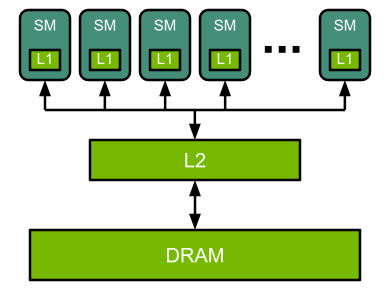
\includegraphics[width=0.70\textwidth]{simple-gpu-arch.png}
	\caption{Memory Hierarchy of the GPU \cite{fig:gpu-arch}}
\end{figure}

Please note that the VRAM is not part of the memory hierarchy, but is
connected to the L2 cache. Caches are used to store frequently used
data and to reduce access times to the main memory. While every SM
has its own L1 cache, the L2 cache is shared between all SMs. Which
means that all cores in one SM are sharing one L1 cache. The CPU
on the other hand has one cache and one memory controller per
core. \cite{CUDA_Programming_Guide}

\section {Summary}

Okay that was a lot of information, so let's summarize the really
important bits what we have learned so far.

The GPU was created to process graphical data much faster than a CPU
could ever do. It allows us to execute the same command on multiple
data simultaneously to prevent waiting for a single command to finish,
which helps us render reaccuring tasks like drawing a texture or model
much faster.  It is made up of many cores which are combined into an
array of streaming multiprocessors (SM) to allow better control and
management of the cores.  The VRAM is the memory of the GPU and its
important to optimize your data to prevent overloading the VRAM.

\chapter {Graphics Rendering Pipeline}

\section {What is the Graphics Pipeline?}

When we talk about the graphics pipeline, I want to make clear that we
are not talking about a physical pipeline that is used to transport data
from one place to another. I've made that mistake when I first started
working with pipelines. My first thought was that the pipeline is a tool
to transport data from the CPU to the GPU, but thats totally wrong.

What is it then? Let's start with a simple definition.

The graphics pipeline is an abstraction layer that is located on the
GPU and is used to process incoming data to create the image that we see
on our screen. \cite{vkGuide} This saves us from writing low level code
explicitly targeting the GPU, which would be a massive task to do.

Please note that the pipeline is implemented differently in every graphics
API, but the basic ideas stay the same. We feed the pipeline with some
graphical data, which then performs operations to transform the data into
an 2D image that can be displayed on our screen. The proccessed data
is then stored in a so called framebuffer, which I will explain later.
\cite{vkGuide}

There is actually other pipeline types, like the compute or raytracing
pipeline, made for different tasks, but we will focus on the graphics
pipeline for now.

The graphics pipeline is invoked by a draw command \cite{build-pipeline},
while the the compute pipeline is invoked by a dispatch
command. \cite{vulkan-tutorial-compute-shader}

\section {Stages of the Pipeline}

The Vulkan pipeline consists of multiple stages. Some of them are fixed
and can not be changed, while others are programmable to act as we
want them to. These changable stages are called shaders and are usually
written in the OpenGL Shading Language (GLSL). These shaders have to be
given to the pipeline as compiled SPIR-V bytecode. \cite{spirv}

Lets take a look at the Vulkan pipeline and its stages:

\begin{figure}[hbtp]
	\centering 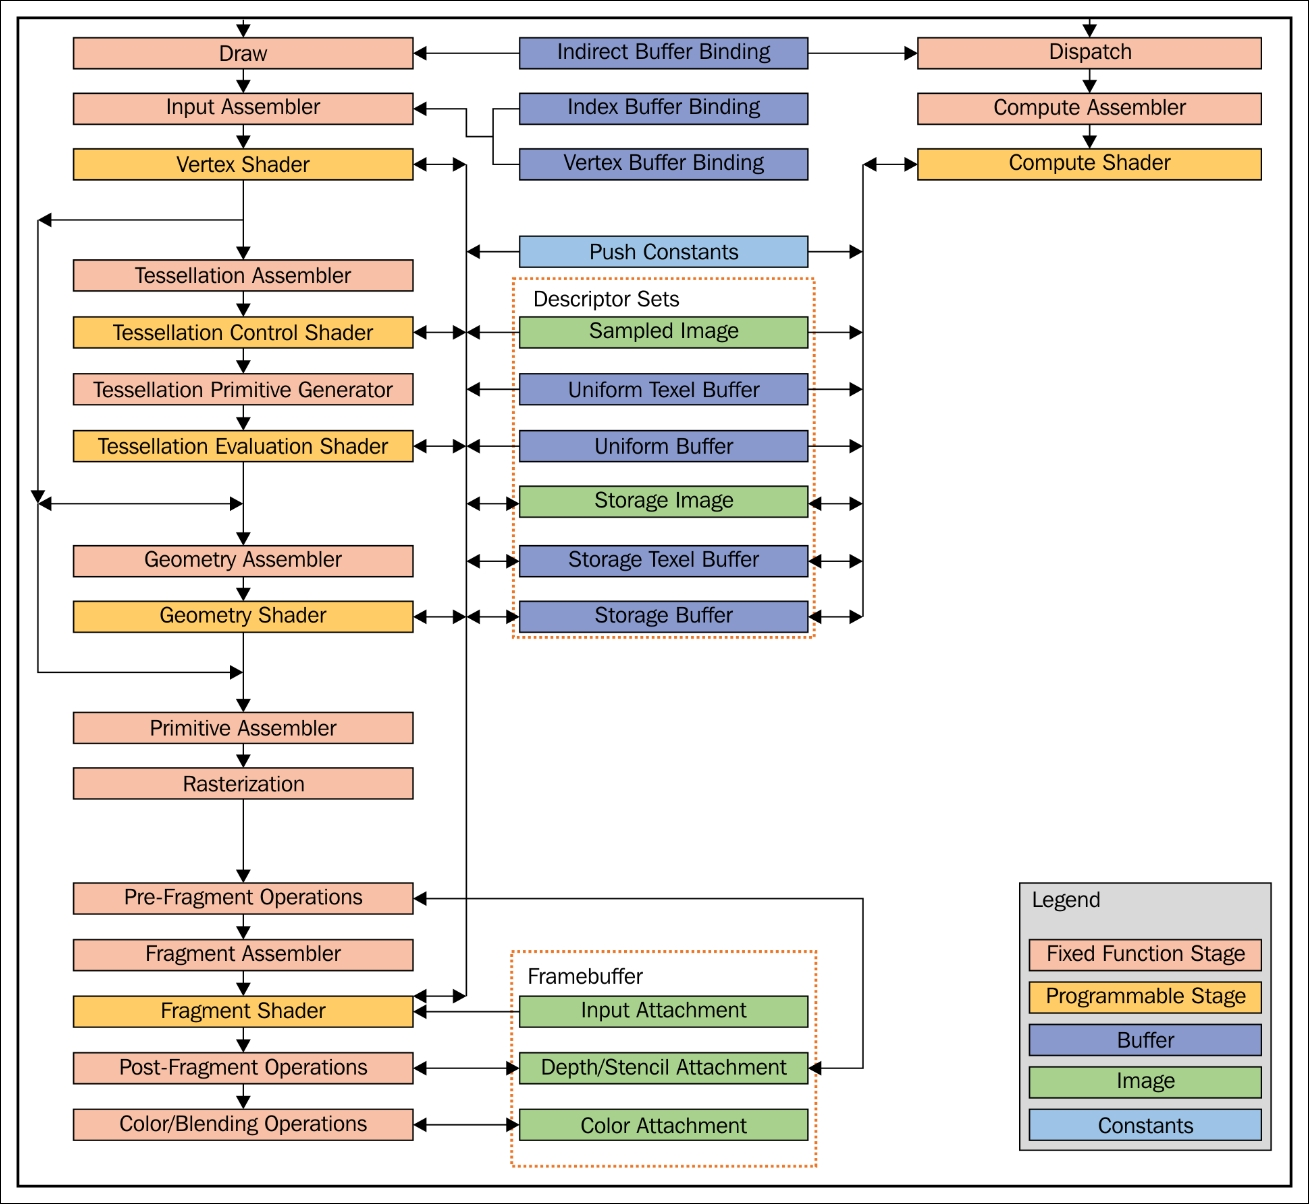
\includegraphics{pipeline.jpg} \caption{Pipeline
		Structure \cite{fig:pipeline}}
\end{figure}

Okay okay, I know thats alot and there is stuff I haven't talked about
yet, like these Buffers, Images and the Push Constants.  Dont worry I
will explain all of these things when going over the stages.

On the left side we have the graphics pipeline and on the right side the
compute pipeline. Now it makes sense that there are different pipelines
for different tasks, right? If we would use the graphics pipeline but
actually just need one shader to edit some data, we would waste a lot
of resources and time sending it though the graphics pipeline.

Im going to focus on the graphics pipeline and its most important stages.
So some stages will be cut short to better explain the important ones.
In the end you will rarely need to use geometry shaders or tessellation
shaders, but it is important to know that they exist and what they do.

\subsection {Draw}

The draw "stage" is not really a stage, but the command that starts
the rendering process. When we call the vkCmdDraw Command on the GPU,
the pipeline will start processing the data that we have given to
it. \cite{vulkan-spec-draw}

\subsection {Input Assembler}

The input assembler is the first stage of the graphics pipeline. It takes
a vertex and index buffer. \cite{vulkan-spec-pipelines} Before we talk
about the input assembler, lets define what a vertex, index and buffer is.

Basically every model that we see is made up of triangles, and vertices
are the corners of these triangles. A single vertex can contain multiple
attributes like position \{x, y, z\}, color \{r, g, b, a\} or texture
coordinates \{u, v\}. \cite{vulkan-vertex-input}

\begin{figure}[hbtp]
	\centering \includesvg[width=0.60\textwidth]{vektor_triangle.svg}
	\caption{Triangle with vertices}
\end{figure} \FloatBarrier

When we want to reuse certain vertices, for example when
drawing a quad, we can add indices.  These indices tell the
input assembler what vertices need to be combined to form a
triangle. \cite{vulkan-tutorial-index-buffer}

For example: A quad has 4 vertices because it has 4 corners. When we want
to draw the quad we have to create two triangles, which means we need 2 *
3 indices.

Vertices: \{0, 1, 2, 3\} Indices: \{\textcolor{red}{0, 1, 2} ,
\textcolor{blue}{0, 2, 3}\}

\begin{figure}[hbtp]
	\centering \includesvg[width=0.50\textwidth]{vi_quad.svg}
	\caption{Quad
		with vertices created using indices}
\end{figure} \FloatBarrier

Here you can see that the first triangle is created by using the vertices
\{\textcolor{red}{0, 1, 2}\} and the second triangle is created by using
the vertices \{\textcolor{blue}{0, 2, 3}\}. I've added the colors just
to clarify which indices are used to create which triangles.

Now that we know what vertices and indices are, we can talk about how we
provide the GPU with this data. There the buffers come into play. A buffer
is basically an array of data that can be bind to the graphics Pipeline.
When the pipeline is created, we need to provide it with the layout of the
buffer, which tells the pipeline how the data in the buffer is structured.
\cite{vulkan-tutorial-vertex-buffer}

In the Vertex Buffer we store the attributes of each vertex as an
array. An attribute can be a position, color or any other related data
of the Vertex. \cite{vulkan-tutorial-vertex-buffer}

\begin{figure}[hbtp]
	\centering \includesvg[width=1\textwidth]{Vertexbuffer.svg}
	\caption{Interleaved Vertex Buffer}
\end{figure} \FloatBarrier

You can see that each attribute has a specific location in the buffer.
These locations tell the pipeline what bytes belong together. So when
accessing the buffers 0. location it gets an vec3(x,y,z).  The pipeline
also needs to know by what offset, in bytes, each vertex is sperated.
In this case it would be 24 bytes, because position and color both
contain 3 floats, which are 4 bytes each. \cite{vulkan-tutorial-vertex-buffer}

This example shows a single buffer containing all atrributes in
an interleaved pattern, but we can also create one buffer for each
attribute and then attach them into a single vertexbuffer. This is called
a non-interleaved pattern.

\begin{figure}[hbtp]
	\includesvg[width=1\textwidth]{non-int-vertexbuffer.svg}
	\caption{Non-Interleaved Vertex Buffer}
\end{figure} \FloatBarrier

Each attribute has has its own binding, to tell the pipeline what location
is assigned to the data. So the first binding will always be the position
until you get to the next binding, which will be the color in this case.
\cite{vulkan-tutorial-vertex-buffer}

Usually we will use interleaved buffers, but in some cases, when we need
different attributes for different tasks, we can use non-interleaved
buffers.

The Indexbuffer on the other hand is just an simple array of integers.
\cite{vulkan-tutorial-index-buffer}

Okay we can now finally talk about the input assembler. The input
assembler takes the vertices and indices to create primitives types like
points, lines or triangles. \cite{microsoft-ia}

\newpage

\begin{lstlisting}[language=C++] 

// Provided by VK_VERSION_1_0 typedef
enum VkPrimitiveTopology {
    VK_PRIMITIVE_TOPOLOGY_POINT_LIST = 0, VK_PRIMITIVE_TOPOLOGY_LINE_LIST
    = 1, VK_PRIMITIVE_TOPOLOGY_LINE_STRIP =
    2, VK_PRIMITIVE_TOPOLOGY_TRIANGLE_LIST =
    3, VK_PRIMITIVE_TOPOLOGY_TRIANGLE_STRIP =
    4, VK_PRIMITIVE_TOPOLOGY_TRIANGLE_FAN = 5,
    VK_PRIMITIVE_TOPOLOGY_LINE_LIST_WITH_ADJACENCY = 6,
    VK_PRIMITIVE_TOPOLOGY_LINE_STRIP_WITH_ADJACENCY = 7,
    VK_PRIMITIVE_TOPOLOGY_TRIANGLE_LIST_WITH_ADJACENCY = 8,
    VK_PRIMITIVE_TOPOLOGY_TRIANGLE_STRIP_WITH_ADJACENCY = 9,
    VK_PRIMITIVE_TOPOLOGY_PATCH_LIST = 10,
} VkPrimitiveTopology; 

\end{lstlisting} \cite{vulkan-spec-primitive-topology}

These are the primitive topology types that the input assembler can
create in Vulkan.  We have to tell the input assembler what type of
topology we want to create, which is usually a triangle strip or list,
but we can also create points or lines.  The difference between a list
and a strip is simple. A list will create a triangle for every 3 indices,
while a strip will create a triangle for every 3 indices and then use
the last 2 vertices of the last triangle to create the next triangle.
The same idea works with lines. The "with adjacency" types are only
used when accessing the geometry stage. We will rarely use
the adjacany types, so dont worry on understanding them now. \cite{vulkan-spec-primitive-topology}

\subsection {Vertex Shader}

The vertex shader is the first programmable stage of the pipeline.


\printbibliography[
	heading=bibintoc, title={Bibliography}
]

\listoffigures

\end {document}
